%!TEX TS-program = xelatex
%!TEX root = ../../maxwell2018thesis.tex

\chapter[Existing Approaches to User Modelling]{Existing Approaches to\\User Modelling}

\section{Individual Components}

\subsection{Query Generation}
Azzopardi, de Rijke
Jordan
Keskustalo, Baskaya...

\subsection{Judging Relevancy}

\subsection{Document Examination}

\section{Entire Search Session}

\subsection{TREC User}

\subsection{Baskaya et al.}

\subsection{Thomas et al.}
\begin{figure}[ht]
	\centering

	\resizebox{1\hsize}{!}{
	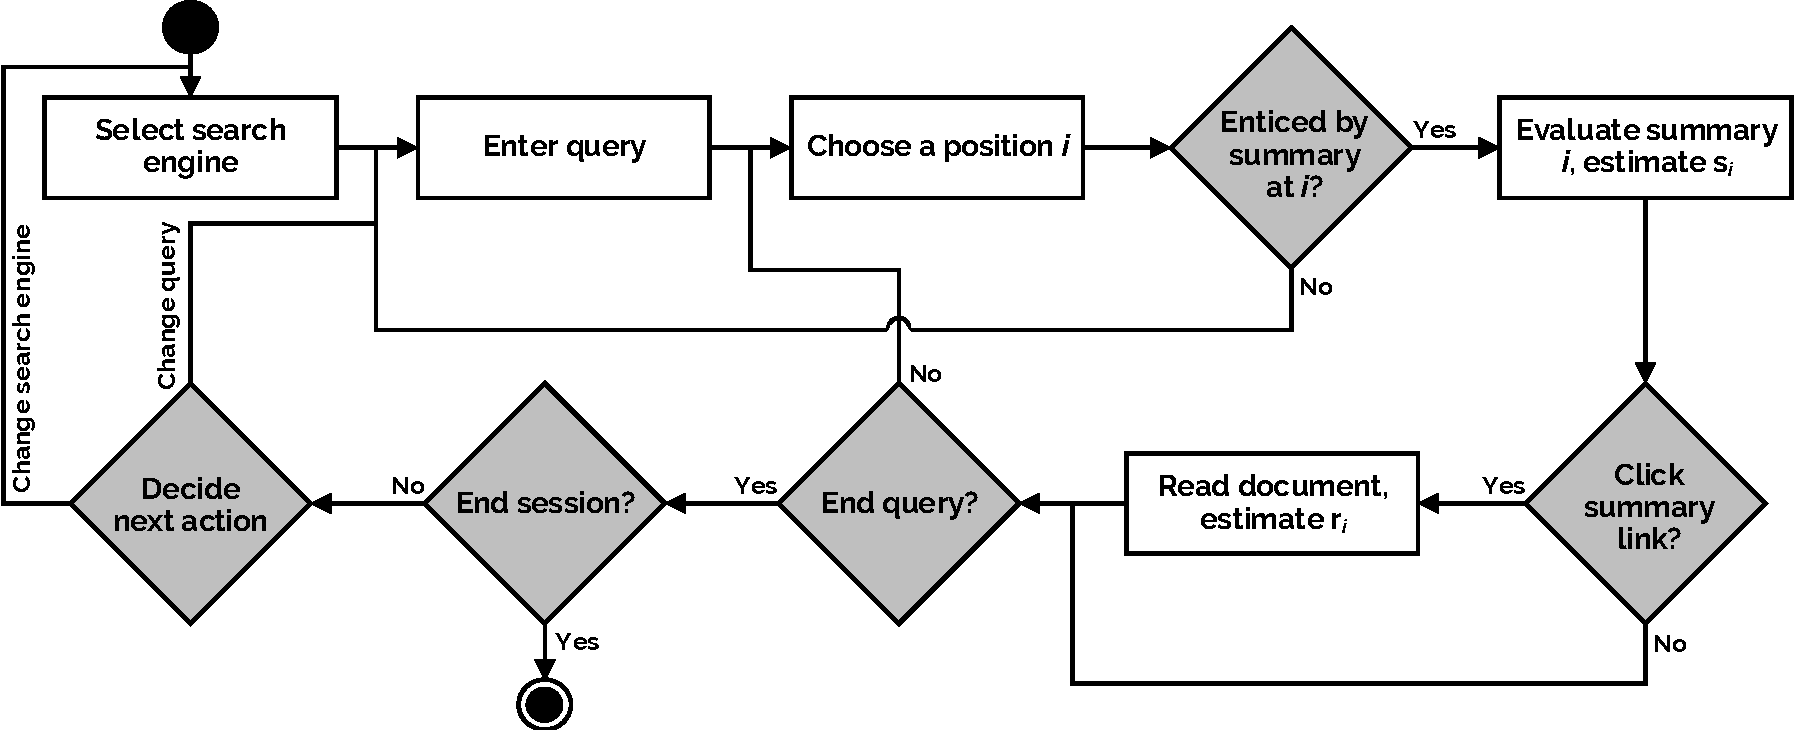
\includegraphics{figures/ch4-thomas_model.pdf}}
	\caption[Interaction model by Thomas et al.]{Model by Thomas et al.}

	\label{fig:ch4-thomas_model}
\end{figure}

\section{Chapter Summary}
- have all these different models